
%(BEGIN_QUESTION)
% Copyright 2012, Tony R. Kuphaldt, released under the Creative Commons Attribution License (v 1.0)
% This means you may do almost anything with this work of mine, so long as you give me proper credit

An {\it unbalanced} wye-connected load receives power from a balanced 120/208 VAC source:

$$\includegraphics[width=15.5cm]{i01044x01.eps}$$

Calculate the current through each of the three lines (L1, L2, and L3), as well as the current through the neutral conductor:

\begin{itemize}
\item{} $I_{L1}$ = \underbar{\hskip 50pt} amps
\vskip 10pt
\item{} $I_{L2}$ = \underbar{\hskip 50pt} amps
\vskip 10pt
\item{} $I_{L3}$ = \underbar{\hskip 50pt} amps
\vskip 10pt
\item{} $I_{N}$ = \underbar{\hskip 50pt} amps
\vskip 10pt
\medskip

\underbar{file i01044}
%(END_QUESTION)





%(BEGIN_ANSWER)

In a 4-wire system such as this, each phase of the load is guaranteed to see the proper (balanced) phase voltage of 120 VAC.  Thus, calculating each line current is the same as calculating each phase (resistor) current as follows:

$$I_{L1} = {120 \over 1500} = 0.08 \hbox{ amps}$$ 

$$I_{L2} = {120 \over 2300} = 0.0522 \hbox{ amps}$$ 

$$I_{L3} = {120 \over 800} = 0.15 \hbox{ amps}$$ 

Neutral conductor current will be the phasor sum of these three phase currents:

$$I_N = I_{L1} + I_{L2} + I_{L3}$$

Of course, we must remember that each of these three currents is phase-shifted from one another by 120 degrees.  Arbitrarily choosing $I_{L1}$ as our zero-degree phase reference, and assuming an L1-L3-L2 rotation:

$$I_N = 0.08 \hbox{ A } \angle 0^o + 0.0522 \hbox{ A } \angle 120^o + 0.15 \hbox{ A } \angle 240^o$$

$$I_N = 0.0873 \hbox{ A } \angle 256^o$$

%(END_ANSWER)





%(BEGIN_NOTES)


%INDEX% Electronics review: 3-phase voltage/current/power calculation

%(END_NOTES)


